\chapter{Using Neural Networks to Enhance COACH}
\section{General Structure}
In previous years, IML techniques were limited to work with low-dimensional state spaces problems and to the use of function approximation such as linear models of basis functions (choosing a right basis function set was crucial for successful learning), in the same way as RL. But, as DRL have showed, by approximating policies with Deep Neural Networks (DNNs) it is possible to solve problems with high-dimensional state spaces, without the need of feature engineering for preprocessing the states. If the same approach is used in IML, the DRL shortcomings mentioned before can be addressed with the support of human users who participate in the learning process of the agent.

This work proposes to extend the use of human corrective feedback during task execution to learn policies with state spaces of low and high dimensionality in continuous action problems (which is the case for most of the problems in robotics) using deep neural networks.

We combine Deep Learning (DL) with the corrective advice based learning framework called COrrective Advice Communicated by Humans (COACH) \cite{Celemin2018AnInteractive}, thus creating the Deep COACH (D-COACH) framework. In this approach, no reward functions are needed and the amount of learning episodes is significantly reduced in comparison to alternative approaches.
\subsection{Replay Buffer}
In D-COACH, the Human Feedback Model is replaced by a memory buffer from which the agent samples past corrections and replays them, in a similar manner as used in DRL problems \cite{atari}. Both the memory buffer and the Human Feedback Model use information given by past corrections to modify the effects of newer ones. Every time feedback is received, the network gets updated by that feedback signal, which is stored in the buffer, and subsequently the network is updated with a batch sampled from the memory buffer. Also, the network gets updated from the buffer with a fixed frequency every $b$ number of time steps.

The policies are updated every time feedback is received and also by sampling from a memory buffer $B$ with a fixed frequency every $b$ time steps. Every time the user advises a correction, the buffer $B$ is fed with the current state and a label generated by adding the action taken with the error correction $y_{label}=a+\mathit{error}$.

\section{Low-dimensional State}

\section{High-dimensional State}
Training CNN policies with human feedback is a challenging problem: both the state representation from raw data (this work focuses on applications that observe raw images), and the policy must be learned with data generated by a human teacher. Deep neural networks have shown to need massive sets of data and experience to adequately converge.  The requirement of massive amounts of trials can be problematic because human users cannot keep on assisting the training for a long time due to stress, fatigue, or other factors that may lead to a lack of concentration.  

To tackle this shortcoming, state representation strategies are employed. The state representation of the policy is trained with additional criteria, adding an autoencoder to help with the training of the convolutional layers (or encoding layers) of the network. 

\subsection{Offline State Learning}
The early version of Deep COACH proposed is a 3-step sequential process. In the first step a session of demonstrations is recorded. Then in a second step, the convolutional layers are trained  with the recorded data, while tuning an  autoencoder  used  for state representation of reduced dimensionality, (Figure \ref{fig:ms}(a)). The state is embedded in the latent space of an autoencoder. Finally, in the third step, the convolutional layers of the trained encoder are frozen, then the subsequent non-convolutional layers (right hand side of Figure \ref{fig:ms}(b)) are trained interactively based on the corrections that the teacher advises to the agent. Figure \ref{fig:ms} depicts the second and third steps of this strategy. 

\begin{figure}
\centering
\subfloat[][Autoencoder network for learning the state representation of the policy based on the demonstrations database.]{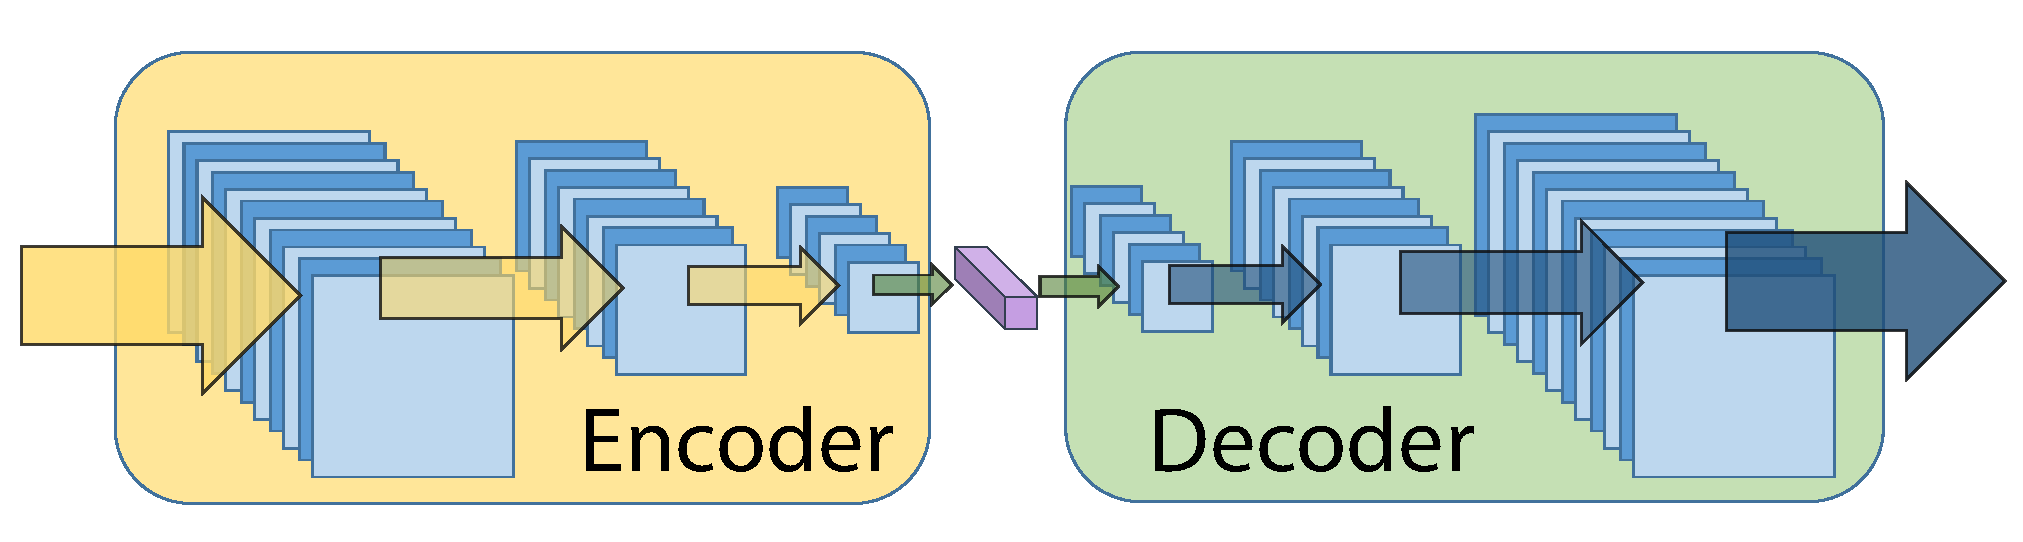
\includegraphics[width=0.45\linewidth]{imagenes/cap2/m1_p1.pdf}}
\hspace{0.1cm}
\subfloat[][Interactive training of the policy using the trained convolutional layers.]{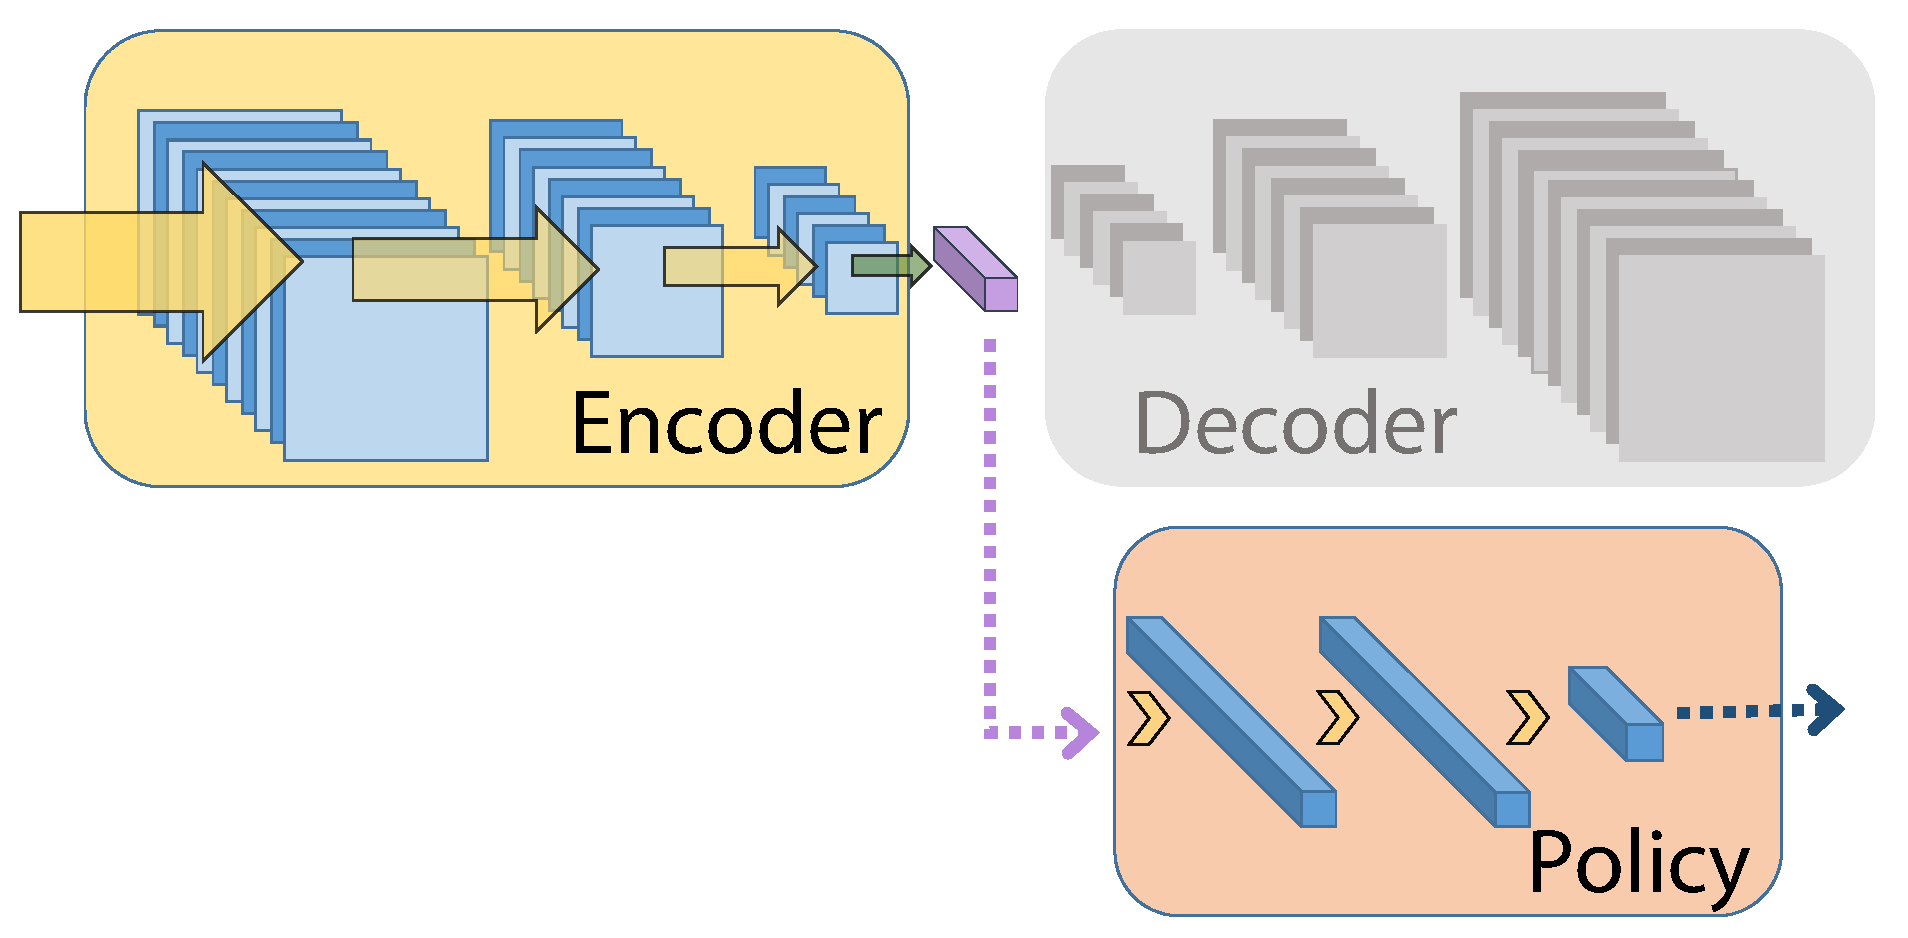
\includegraphics[width=0.45\linewidth]{imagenes/cap2/m1_p2.pdf}}
\caption{D-COACH offline state learning.} 
\label{fig:ms} 
\end{figure}

This kind of sequential strategy has been proven to work in decision-making problems \cite{Warnell2017,Finn2015,Ha2018}, but, it has the shortcoming that it needs a database with images of the environment to work. This can be time consuming and not robust to changes in the environment. In Algorithm \ref{algorithm:DeepCOACH}, the pseudocode of the offline state learning version of D-COACH is presented.

\begin{algorithm}[t]
\caption{D-COACH }\label{algorithm:DeepCOACH}
\begin{algorithmic}[1]
\State \textbf{Require:} error magnitude $e$, buffer update interval $b$, buffer sampling size $N$, buffer size $K$, pre-trained encoder parameters (if convolutional) 
\State \textbf{Init:} $B = []$  \emph{\# initialize memory buffer}
\For{t = 1,2,...}{}
\State \textbf{observe} state $s_{t}$
\State \textbf{execute} action $a_{t}=\pi(s)_{t}$
\State \textbf{feedback} human corrective advice $h_{t}$
\If{$h_{t}$ is not \textbf{0}}
\State $\mathit{error}_{t} = h_{t}\cdot e$
\State $y_{label(t)} = a_{t} + \mathit{error}_{t}$ 
\State \textbf{update} $\pi(s)$ using SGD with pair ($s_{t}$, $y_{\mathit{label}(t)}$) 
\State \textbf{update} $\pi(s)$ using SGD with a mini-batch sampled from $B$
\State \textbf{append} $(s_{t}, y_{\mathit{label}(t)})$ to $B$
\If{length($B$) $> K$ }
\State $B = B[2:K+1]$
\EndIf
\EndIf
\If{mod(t, b) is 0 and $B$ is not $\emptyset$}
\State \textbf{compute} $\pi(s)$ using SGD with a mini-batch sampled from $B$
\EndIf
\EndFor
\end{algorithmic}
\end{algorithm}

\subsection{Online State Learning}
In order to eliminate the requirement of recording demonstrations and pre-training an autoencoder, an enhanced version of Deep COACH is proposed, which learns everything in a single step of interaction, as the original COACH does. Hence, it allows to train all the parameters of the network interactively from scratch. State representation strategies have been included in order to make the networks converge faster. The basic idea is to train the state representation of the policy with additional auxiliary criteria (autoencoding). So, in addition to the loss function for predicting the policy based on the data generated by the human corrections, it also includes the loss function of the reconstruction at the output of the autoencoder, based on the same data stored during the human corrections. 

Both networks, the policy and the autoencoder, share the convolutional layers of the encoder as shown in Figure \ref{fig:msim}. The policy network has the convolutional layers at the input, followed by a second part that is a fully connected layer, then this network maps from STATE to ACTION, while the autoencoder network involves the computation from STATE to STATE$*$, wherein  STATE$*$ is the reconstructed image at the output of the decoder, according to Figure \ref{fig:msim}.

\begin{figure}[H]
    \centering
    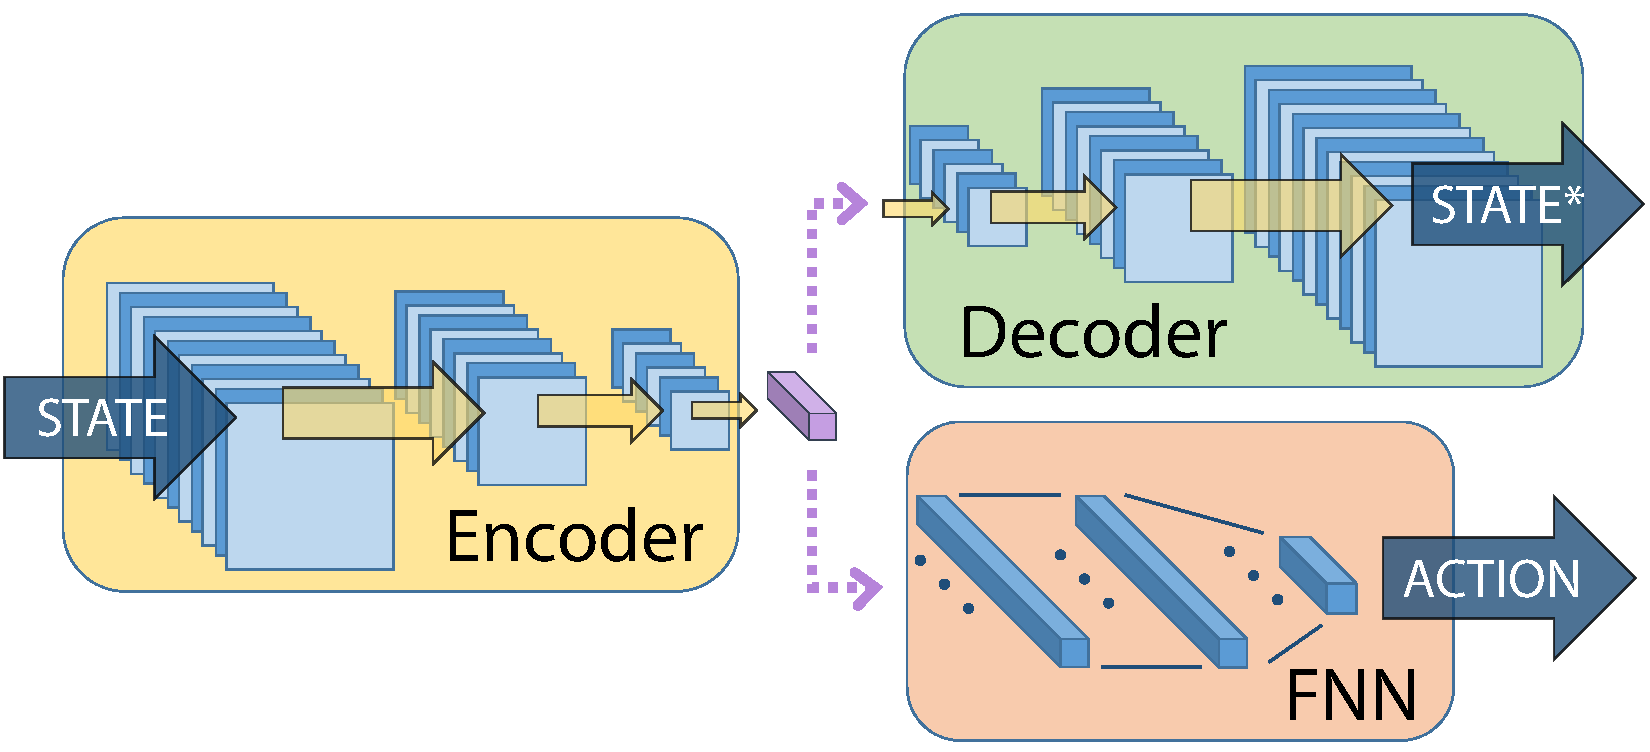
\includegraphics[width=0.6\linewidth]{imagenes/cap2/m2.pdf}
    \caption{D-COACH online state learning. The state representation is shared between the autoencoder and the policy training.}
    \label{fig:msim}
\end{figure}

Algorithm \ref{algorithm:DeepCOACH} describes the enhanced version of D-COACH. The algorithm first sets the hyper-parameters like the magnitude of the error \eqref{eq:error}, and the ones used for the corrections replay. Line 4 to 18 shows the algorithm that is executed every time step. In cases when the teacher advises a correction in line 6, the subsequent lines are evaluated, wherein the policy network is updated along with the autoencoder network, and the buffer of state-action pairs for the corrections replay process.
Two different updates are computed, one for the layers involved in the policy computation, and another for the layers of the autoencoder. When an advice of correction is given, first, the \textbf{update} $policy$ instruction updates the policy network for the current state, and also with a mini-batch sampled from the corrections buffer. 

For the corrections replay process, the \textbf{update} $policy$ is run every $b$ time steps. Also, if the reconstruction error of the autoencoder (difference between STATE and STATE$*$) is greater than a threshold $\epsilon$ (line 17), the autoencoder is updated with the same mini-batch using the instruction \textbf{update} $AE$ ($Autoencoder$). Otherwise the convolutional layers are frozen, so the instruction \textbf{update} $policy$ in lines 10, 11, and 16, would modify only the non-convolutional layers with the Stochastic Gradient Descent (SGD) operation. The \textbf{update} $policy$ instruction uses the [state,$y_{label}$] pairs of the mini-batch, whereas \textbf{update} $AE$ only uses the states. The aforementioned condition in line 17 is used for avoiding conflicts in the gradients of both cost functions, so when the latent vector of the (AE) is considered a good smaller representation of the state, the gradient of the policy must be prevented from harming the learned encoding. Hence, the encoder is kept frozen, unless unknown regions of the state space are visited.

\begin{algorithm}[t]
\caption{D-COACH }\label{algorithm:DeepCOACH}
\begin{algorithmic}[1]
\State \textbf{Require:} error magnitude $\textit{e}$, buffer update interval $b$, buffer sampling size $N$, buffer size $K$, pre-trained encoder parameters (if 3-step sequential learning) 
\State \textbf{Init:} $B = []$ \emph{\# initialize memory buffer}
\For{t = 1,2,...}{}
\State \textbf{observe} state $s_{t}$
\State \textbf{execute} action $a_{t}=\pi(s)_{t}$
\State \textbf{feedback} human corrective advice $h_{t}$
\If{$h_{t}$ is not \textbf{0}}
\State $error_{t} = h_{t}\cdot e$
\State $y_{label(t)} = a_{t} + error_{t}$ 
\State \textbf{update} $policy$ using SGD with pair ($s_{t}$, $y_{label(t)}$) 
\State \textbf{update} $policy$ using SGD with a mini-batch sampled from $B$
\State \textbf{append} $(s_{t}, y_{label(t)})$ to $B$
\If{length($B$) $> K$ }
\State $B = B[2:K+1]$
\EndIf
\EndIf
\If{mod(t, b) is 0 and $B$ is not $\emptyset$}
\State \textbf{update} $policy$ using SGD with a mini-batch sampled from $B$
\If{$AE_{error}>\epsilon$  }
\State \textbf{update} $AE$ using SGD with a mini-batch sampled from $B$
\State \textbf{unfreeze} convolutional layers
\Else
\State \textbf{freeze} convolutional layers
\EndIf
\EndIf
\EndFor
\end{algorithmic}
\end{algorithm}

\section{Partially Observed Problems}
\subsection{Adding Memory to the Network}
\subsubsection{Low-dimensional State with Memory}
\subsubsection{High-dimensional State with Memory}

\section{Exploiting Correlations in the Action Space}
In the original COACH, it is proposed that each dimension should be trained independently \cite{Celemin2017}, which has the advantage of creating a working framework that does not need any prior information about the problem in order to give corrections. We call this type of policy updating \emph{decoupled} training, so a correction in an specific action dimension does not modify the magnitude of the actions in other axes for the same corresponding state. However, in this work we consider that for some problems it may be advantageous to exploit prior user knowledge about relations between the different dimensions of the actions. In this way, a correction in one of the action axes may be used to update more than one dimension. We call this case \emph{coupled} training.